\hypertarget{interface_8cpp}{}\section{O\+L13/interface.cpp File Reference}
\label{interface_8cpp}\index{O\+L13/interface.\+cpp@{O\+L13/interface.\+cpp}}


//\+Expliquer brievement à quoi sert ce fichier. //\+EX \+: Définit les modèles de voiture et leur particularités.  


{\ttfamily \#include \char`\"{}interface.\+h\char`\"{}}\newline
Include dependency graph for interface.\+cpp\+:\nopagebreak
\begin{figure}[H]
\begin{center}
\leavevmode
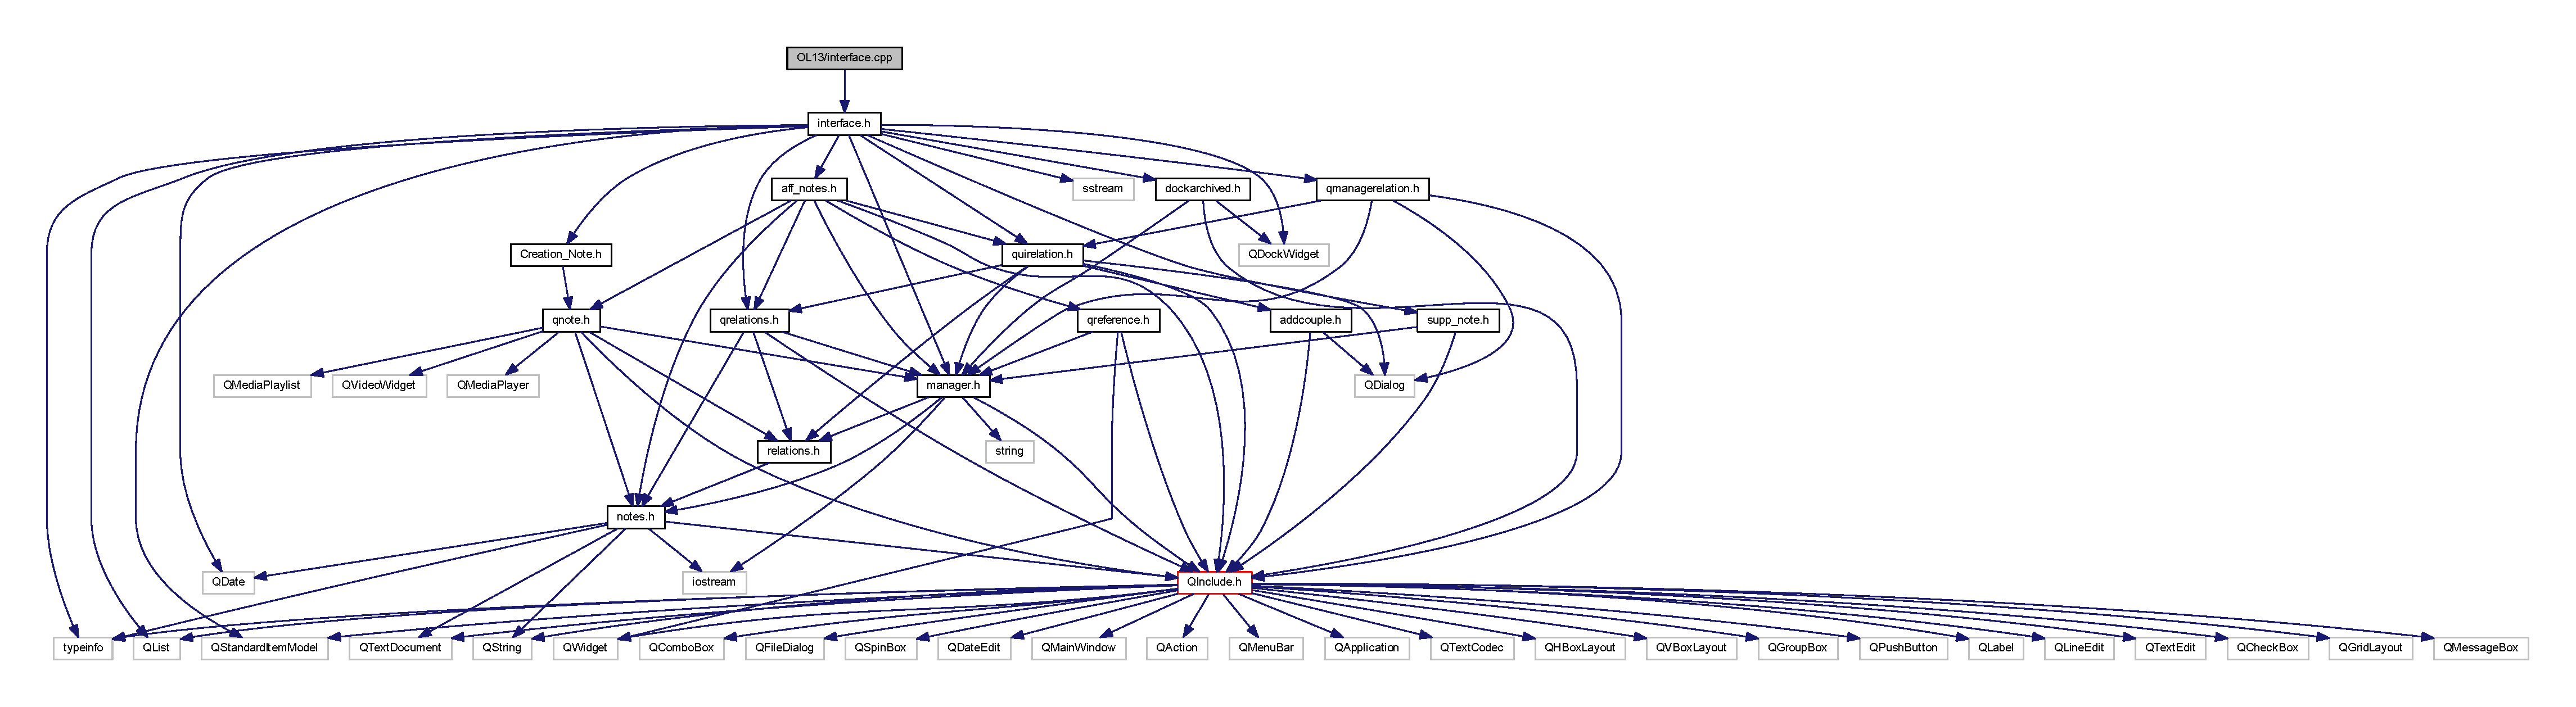
\includegraphics[width=350pt]{interface_8cpp__incl}
\end{center}
\end{figure}


\subsection{Detailed Description}
//\+Expliquer brievement à quoi sert ce fichier. //\+EX \+: Définit les modèles de voiture et leur particularités. 

\begin{DoxyAuthor}{Author}
Garnier Maxime, Naudin Louise, Pépin Hugues 
\end{DoxyAuthor}
\begin{DoxyVersion}{Version}
1.\+0 
\end{DoxyVersion}
\begin{DoxyDate}{Date}
14 Juin 2017
\end{DoxyDate}
//\+Expliquer en détail. //\+EX \+:Cette classe surcharge les accesseurs standards du module\+\_\+voiture pour convenir aux spécificités des différents modèles possibles. 